Here is the method used to examine the question

\section{Synthetic Data Sets}
The initial experiments in this study are performed on synthetic data obtained through rendering of a 3D head model in a data generation framework. This framework is based on the work of \textcite{swirski2014rendering} and utilizes the same head rig. Two data sets with resolution 256x256 was generated. For reproducability, the data sets will become publicly available at the time of publication.

The synthetic data sets are fully annotated with automatically generated ground truth labels. The relevant labels for the experiments are converted to heatmaps when loaded for training and evaluation as in most cases of semantic segmentation \parencite{guo2017review}. These heatmaps are thereafter concatenated with the real images, forming feature maps of shape 2x320x320. By viewing the annotations as a part of the data, unsupervised models that learn the data distribution implicitly learn the relations between the annotations and the images.

\section{Network architectures}
...relevant network architectures are described here, together with figures and stuff. Base it around GAN networks, the small differences in the encoders can be explained afterwards.

\section{\acrlong{vaes}}
A \acrlong{vae} was constructed and trained on the synthetic data as a baseline for further experiments. The advantages of using \acrshort{vaes} for data generation in contrast to \acrshort{gans} is that they are easier to train and does not suffer from vanishing modes of data.


\section{Progressive \acrshort{gan}}
The first method tested in this project was the progressive \acrshort{gan}, proposed by \textcite{karras2017progressive}. The proposed advantages of this approach over other existing acrshort{gan} variations is two-fold. Firstly, there is reason to believe that the quality and diversity of the generated samples are improved by the progressive training. Secondly, the training stability is believed to increase. However due to the novelty of the approach and the lack of extensive evaluations of different \acrshort{gans} it is difficult to know for sure if this is the case.

It was adopted because of the proposed training stability that arises from progressivly increasing the complexity of the learned task. 

\subsection{Freeze in new layers}

\begin{figure}[t]
    \centering
    \begin{subfigure}[b]{0.45\textwidth}
        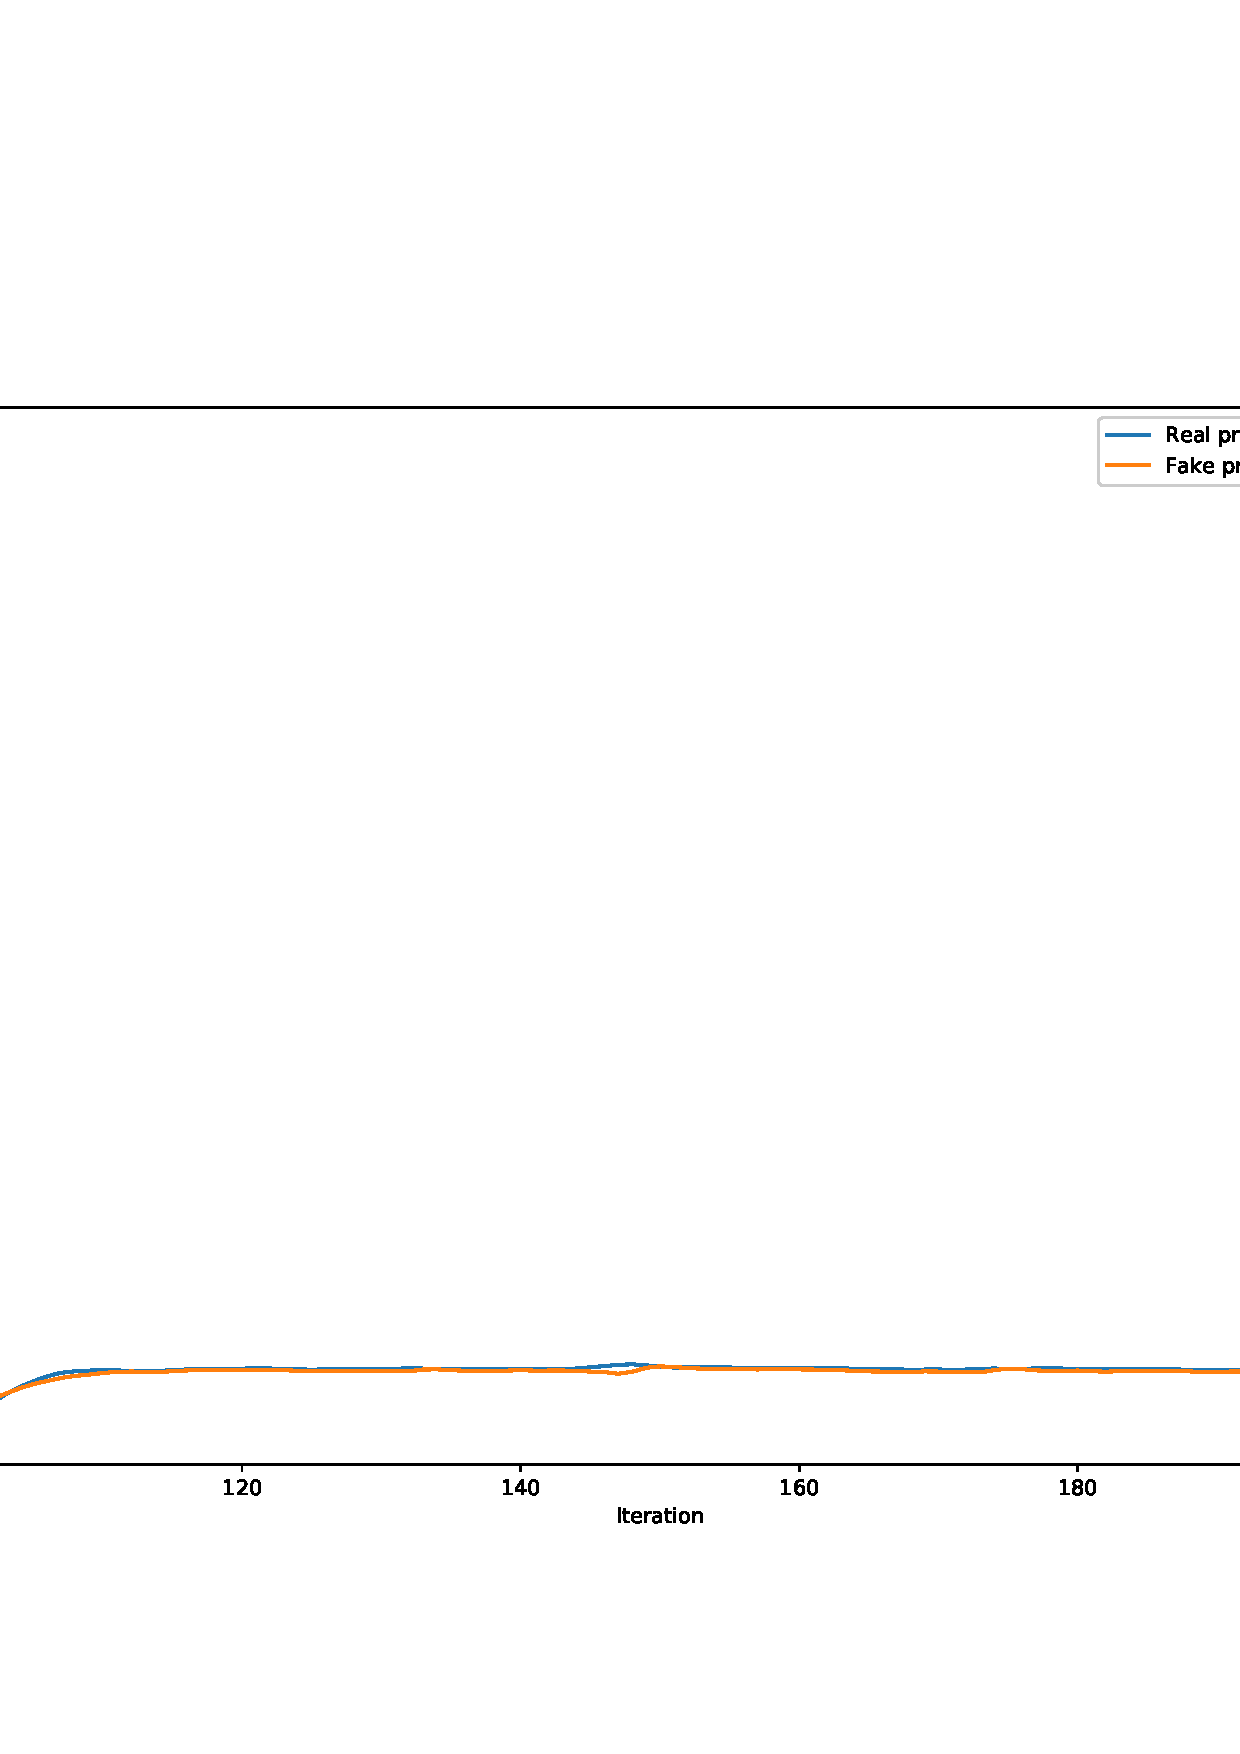
\includegraphics[width=\textwidth]{results/freezeInDG1.png}
        \caption{Yo flo}
        \label{fig:freezeInDG1}
    \end{subfigure}
    \begin{subfigure}[b]{0.45\textwidth}
        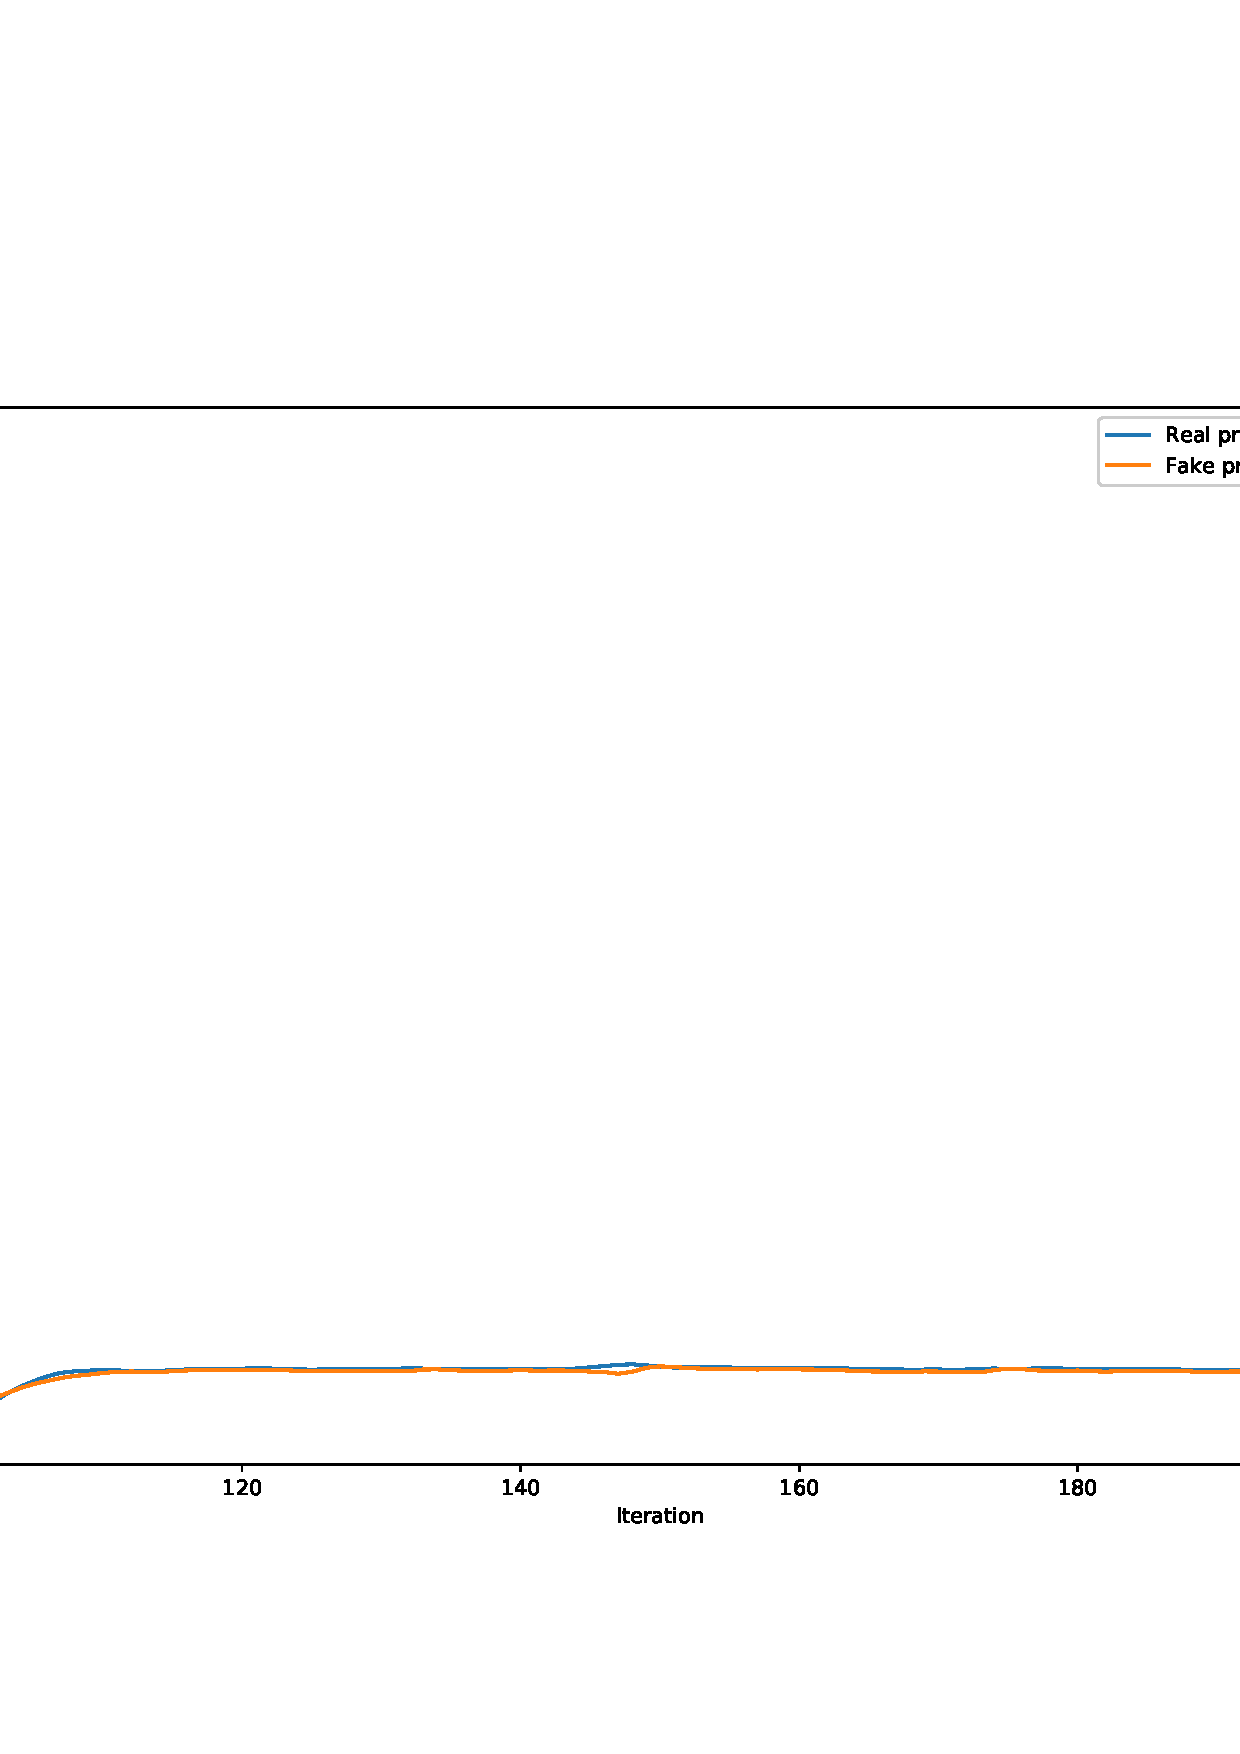
\includegraphics[width=\textwidth]{results/freezeInDG1.png}
        \caption{Yo flo}
        \label{fig:freezeInDG2}
    \end{subfigure}
    \caption{Yo yo yo}
    \label{fig:fadeVsFreeze}
\end{figure}



\section{VAE initialization}


